
%% bare_conf.tex
%% V1.4b
%% 2015/08/26
%% by Michael Shell
%% See:
%% http://www.michaelshell.org/
%% for current contact information.
%%
%% This is a skeleton file demonstrating the use of IEEEtran.cls
%% (requires IEEEtran.cls version 1.8b or later) with an IEEE
%% conference paper.
%%
%% Support sites:
%% http://www.michaelshell.org/tex/ieeetran/
%% http://www.ctan.org/pkg/ieeetran
%% and
%% http://www.ieee.org/

%%*************************************************************************
%% Legal Notice:
%% This code is offered as-is without any warranty either expressed or
%% implied; without even the implied warranty of MERCHANTABILITY or
%% FITNESS FOR A PARTICULAR PURPOSE!
%% User assumes all risk.
%% In no event shall the IEEE or any contributor to this code be liable for
%% any damages or losses, including, but not limited to, incidental,
%% consequential, or any other damages, resulting from the use or misuse
%% of any information contained here.
%%
%% All comments are the opinions of their respective authors and are not
%% necessarily endorsed by the IEEE.
%%
%% This work is distributed under the LaTeX Project Public License (LPPL)
%% ( http://www.latex-project.org/ ) version 1.3, and may be freely used,
%% distributed and modified. A copy of the LPPL, version 1.3, is included
%% in the base LaTeX documentation of all distributions of LaTeX released
%% 2003/12/01 or later.
%% Retain all contribution notices and credits.
%% ** Modified files should be clearly indicated as such, including  **
%% ** renaming them and changing author support contact information. **
%%*************************************************************************


% *** Authors should verify (and, if needed, correct) their LaTeX system  ***
% *** with the testflow diagnostic prior to trusting their LaTeX platform ***
% *** with production work. The IEEE's font choices and paper sizes can   ***
% *** trigger bugs that do not appear when using other class files.       ***                          ***
% The testflow support page is at:
% http://www.michaelshell.org/tex/testflow/



\documentclass[conference]{IEEEtran}
% Some Computer Society conferences also require the compsoc mode option,
% but others use the standard conference format.
%
% If IEEEtran.cls has not been installed into the LaTeX system files,
% manually specify the path to it like:
% \documentclass[conference]{../sty/IEEEtran}





% Some very useful LaTeX packages include:
% (uncomment the ones you want to load)


% *** MISC UTILITY PACKAGES ***
%
%\usepackage{ifpdf}
% Heiko Oberdiek's ifpdf.sty is very useful if you need conditional
% compilation based on whether the output is pdf or dvi.
% usage:
% \ifpdf
%   % pdf code
% \else
%   % dvi code
% \fi
% The latest version of ifpdf.sty can be obtained from:
% http://www.ctan.org/pkg/ifpdf
% Also, note that IEEEtran.cls V1.7 and later provides a builtin
% \ifCLASSINFOpdf conditional that works the same way.
% When switching from latex to pdflatex and vice-versa, the compiler may
% have to be run twice to clear warning/error messages.






% *** CITATION PACKAGES ***
%
%\usepackage{cite}
% cite.sty was written by Donald Arseneau
% V1.6 and later of IEEEtran pre-defines the format of the cite.sty package
% \cite{} output to follow that of the IEEE. Loading the cite package will
% result in citation numbers being automatically sorted and properly
% "compressed/ranged". e.g., [1], [9], [2], [7], [5], [6] without using
% cite.sty will become [1], [2], [5]--[7], [9] using cite.sty. cite.sty's
% \cite will automatically add leading space, if needed. Use cite.sty's
% noadjust option (cite.sty V3.8 and later) if you want to turn this off
% such as if a citation ever needs to be enclosed in parenthesis.
% cite.sty is already installed on most LaTeX systems. Be sure and use
% version 5.0 (2009-03-20) and later if using hyperref.sty.
% The latest version can be obtained at:
% http://www.ctan.org/pkg/cite
% The documentation is contained in the cite.sty file itself.






% *** GRAPHICS RELATED PACKAGES ***
%
\ifCLASSINFOpdf
  % \usepackage[pdftex]{graphicx}
  % declare the path(s) where your graphic files are
  % \graphicspath{{../pdf/}{../jpeg/}}
  % and their extensions so you won't have to specify these with
  % every instance of \includegraphics
  % \DeclareGraphicsExtensions{.pdf,.jpeg,.png}
\else
  % or other class option (dvipsone, dvipdf, if not using dvips). graphicx
  % will default to the driver specified in the system graphics.cfg if no
  % driver is specified.
  % \usepackage[dvips]{graphicx}
  % declare the path(s) where your graphic files are
  % \graphicspath{{../eps/}}
  % and their extensions so you won't have to specify these with
  % every instance of \includegraphics
  % \DeclareGraphicsExtensions{.eps}
\fi
% graphicx was written by David Carlisle and Sebastian Rahtz. It is
% required if you want graphics, photos, etc. graphicx.sty is already
% installed on most LaTeX systems. The latest version and documentation
% can be obtained at:
% http://www.ctan.org/pkg/graphicx
% Another good source of documentation is "Using Imported Graphics in
% LaTeX2e" by Keith Reckdahl which can be found at:
% http://www.ctan.org/pkg/epslatex
%
% latex, and pdflatex in dvi mode, support graphics in encapsulated
% postscript (.eps) format. pdflatex in pdf mode supports graphics
% in .pdf, .jpeg, .png and .mps (metapost) formats. Users should ensure
% that all non-photo figures use a vector format (.eps, .pdf, .mps) and
% not a bitmapped formats (.jpeg, .png). The IEEE frowns on bitmapped formats
% which can result in "jaggedy"/blurry rendering of lines and letters as
% well as large increases in file sizes.
%
% You can find documentation about the pdfTeX application at:
% http://www.tug.org/applications/pdftex





% *** MATH PACKAGES ***
%
%\usepackage{amsmath}
% A popular package from the American Mathematical Society that provides
% many useful and powerful commands for dealing with mathematics.
%
% Note that the amsmath package sets \interdisplaylinepenalty to 10000
% thus preventing page breaks from occurring within multiline equations. Use:
%\interdisplaylinepenalty=2500
% after loading amsmath to restore such page breaks as IEEEtran.cls normally
% does. amsmath.sty is already installed on most LaTeX systems. The latest
% version and documentation can be obtained at:
% http://www.ctan.org/pkg/amsmath





% *** SPECIALIZED LIST PACKAGES ***
%
%\usepackage{algorithmic}
% algorithmic.sty was written by Peter Williams and Rogerio Brito.
% This package provides an algorithmic environment fo describing algorithms.
% You can use the algorithmic environment in-text or within a figure
% environment to provide for a floating algorithm. Do NOT use the algorithm
% floating environment provided by algorithm.sty (by the same authors) or
% algorithm2e.sty (by Christophe Fiorio) as the IEEE does not use dedicated
% algorithm float types and packages that provide these will not provide
% correct IEEE style captions. The latest version and documentation of
% algorithmic.sty can be obtained at:
% http://www.ctan.org/pkg/algorithms
% Also of interest may be the (relatively newer and more customizable)
% algorithmicx.sty package by Szasz Janos:
% http://www.ctan.org/pkg/algorithmicx




% *** ALIGNMENT PACKAGES ***
%
%\usepackage{array}
% Frank Mittelbach's and David Carlisle's array.sty patches and improves
% the standard LaTeX2e array and tabular environments to provide better
% appearance and additional user controls. As the default LaTeX2e table
% generation code is lacking to the point of almost being broken with
% respect to the quality of the end results, all users are strongly
% advised to use an enhanced (at the very least that provided by array.sty)
% set of table tools. array.sty is already installed on most systems. The
% latest version and documentation can be obtained at:
% http://www.ctan.org/pkg/array


% IEEEtran contains the IEEEeqnarray family of commands that can be used to
% generate multiline equations as well as matrices, tables, etc., of high
% quality.




% *** SUBFIGURE PACKAGES ***
%\ifCLASSOPTIONcompsoc
%  \usepackage[caption=false,font=normalsize,labelfont=sf,textfont=sf]{subfig}
%\else
%  \usepackage[caption=false,font=footnotesize]{subfig}
%\fi
% subfig.sty, written by Steven Douglas Cochran, is the modern replacement
% for subfigure.sty, the latter of which is no longer maintained and is
% incompatible with some LaTeX packages including fixltx2e. However,
% subfig.sty requires and automatically loads Axel Sommerfeldt's caption.sty
% which will override IEEEtran.cls' handling of captions and this will result
% in non-IEEE style figure/table captions. To prevent this problem, be sure
% and invoke subfig.sty's "caption=false" package option (available since
% subfig.sty version 1.3, 2005/06/28) as this is will preserve IEEEtran.cls
% handling of captions.
% Note that the Computer Society format requires a larger sans serif font
% than the serif footnote size font used in traditional IEEE formatting
% and thus the need to invoke different subfig.sty package options depending
% on whether compsoc mode has been enabled.
%
% The latest version and documentation of subfig.sty can be obtained at:
% http://www.ctan.org/pkg/subfig




% *** FLOAT PACKAGES ***
%
%\usepackage{fixltx2e}
% fixltx2e, the successor to the earlier fix2col.sty, was written by
% Frank Mittelbach and David Carlisle. This package corrects a few problems
% in the LaTeX2e kernel, the most notable of which is that in current
% LaTeX2e releases, the ordering of single and double column floats is not
% guaranteed to be preserved. Thus, an unpatched LaTeX2e can allow a
% single column figure to be placed prior to an earlier double column
% figure.
% Be aware that LaTeX2e kernels dated 2015 and later have fixltx2e.sty's
% corrections already built into the system in which case a warning will
% be issued if an attempt is made to load fixltx2e.sty as it is no longer
% needed.
% The latest version and documentation can be found at:
% http://www.ctan.org/pkg/fixltx2e


%\usepackage{stfloats}
% stfloats.sty was written by Sigitas Tolusis. This package gives LaTeX2e
% the ability to do double column floats at the bottom of the page as well
% as the top. (e.g., "\begin{figure*}[!b]" is not normally possible in
% LaTeX2e). It also provides a command:
%\fnbelowfloat
% to enable the placement of footnotes below bottom floats (the standard
% LaTeX2e kernel puts them above bottom floats). This is an invasive package
% which rewrites many portions of the LaTeX2e float routines. It may not work
% with other packages that modify the LaTeX2e float routines. The latest
% version and documentation can be obtained at:
% http://www.ctan.org/pkg/stfloats
% Do not use the stfloats baselinefloat ability as the IEEE does not allow
% \baselineskip to stretch. Authors submitting work to the IEEE should note
% that the IEEE rarely uses double column equations and that authors should try
% to avoid such use. Do not be tempted to use the cuted.sty or midfloat.sty
% packages (also by Sigitas Tolusis) as the IEEE does not format its papers in
% such ways.
% Do not attempt to use stfloats with fixltx2e as they are incompatible.
% Instead, use Morten Hogholm'a dblfloatfix which combines the features
% of both fixltx2e and stfloats:
%
% \usepackage{dblfloatfix}
% The latest version can be found at:
% http://www.ctan.org/pkg/dblfloatfix




% *** PDF, URL AND HYPERLINK PACKAGES ***
%
%\usepackage{url}
% url.sty was written by Donald Arseneau. It provides better support for
% handling and breaking URLs. url.sty is already installed on most LaTeX
% systems. The latest version and documentation can be obtained at:
% http://www.ctan.org/pkg/url
% Basically, \url{my_url_here}.




% *** Do not adjust lengths that control margins, column widths, etc. ***
% *** Do not use packages that alter fonts (such as pslatex).         ***
% There should be no need to do such things with IEEEtran.cls V1.6 and later.
% (Unless specifically asked to do so by the journal or conference you plan
% to submit to, of course. )


% correct bad hyphenation here
\hyphenation{op-tical net-works semi-conduc-tor}


\begin{document}
%
% paper title
% Titles are generally capitalized except for words such as a, an, and, as,
% at, but, by, for, in, nor, of, on, or, the, to and up, which are usually
% not capitalized unless they are the first or last word of the title.
% Linebreaks \\ can be used within to get better formatting as desired.
% Do not put math or special symbols in the title.
\title{Bare Demo of IEEEtran.cls\\ for IEEE Conferences}


% author names and affiliations
% use a multiple column layout for up to three different
% affiliations
\author{\IEEEauthorblockN{Murat Ambarkutuk}
\IEEEauthorblockA{
Mechanical Engineering Department, \\
Virginia Polytechnic Institute and State University, \\
Blacksburg, Virginia, USA
Email:murata@vt.edu
}\and
\IEEEauthorblockN{Tomonari Furukawa}
\IEEEauthorblockA{
Mechanical Engineering Department, \\
Virginia Polytechnic Institute and State University, \\
Blacksburg, Virginia, USA
Email: tomonari@vt.edu
}}

% conference papers do not typically use \thanks and this command
% is locked out in conference mode. If really needed, such as for
% the acknowledgment of grants, issue a \IEEEoverridecommandlockouts
% after \documentclass

% for over three affiliations, or if they all won't fit within the width
% of the page, use this alternative format:
%
%\author{\IEEEauthorblockN{Michael Shell\IEEEauthorrefmark{1},
%Homer Simpson\IEEEauthorrefmark{2},
%James Kirk\IEEEauthorrefmark{3},
%Montgomery Scott\IEEEauthorrefmark{3} and
%Eldon Tyrell\IEEEauthorrefmark{4}}
%\IEEEauthorblockA{\IEEEauthorrefmark{1}School of Electrical and Computer Engineering\\
%Georgia Institute of Technology,
%Atlanta, Georgia 30332--0250\\ Email: see http://www.michaelshell.org/contact.html}
%\IEEEauthorblockA{\IEEEauthorrefmark{2}Twentieth Century Fox, Springfield, USA\\
%Email: homer@thesimpsons.com}
%\IEEEauthorblockA{\IEEEauthorrefmark{3}Starfleet Academy, San Francisco, California 96678-2391\\
%Telephone: (800) 555--1212, Fax: (888) 555--1212}
%\IEEEauthorblockA{\IEEEauthorrefmark{4}Tyrell Inc., 123 Replicant Street, Los Angeles, California 90210--4321}}




% use for special paper notices
%\IEEEspecialpapernotice{(Invited Paper)}




% make the title area
\maketitle

% As a general rule, do not put math, special symbols or citations
% in the abstract
\begin{abstract}
    This paper presents a robot localization system with WiFi signal where a Deep Learning framework utilized to fully exploit the information from signal maps of various Access Points (AP) available in an environment.
    Similar to conventional systems relying on the fingerprinting technique, the system is consisted of two stages: data acquisition and learning (offline), and localization (online).
    In offline stage, the signal maps for various AP's are constructed via Received Signal Strength (RSS) information and learned by a Convolutional Neural Network, whereas the online stage contains the proposed localization method based on an information fusion technique.
    \textit{Add some result once get it}
\end{abstract}

% no keywords




% For peer review papers, you can put extra information on the cover
% page as needed:
% \ifCLASSOPTIONpeerreview
% \begin{center} \bfseries EDICS Category: 3-BBND \end{center}
% \fi
%
% For peerreview papers, this IEEEtran command inserts a page break and
% creates the second title. It will be ignored for other modes.
\IEEEpeerreviewmaketitle



\section{Introduction}

  Since WiFi has become ubiquitious, it started being utilized in different applications varying from customer tracking indoors to robot localization. % more varying examples would be good.
  However it is available, the information can be extracted from is prone to (suffers from) being sparse and severely effected by infrasracture of environments where WiFi based systems are deployed.
  Amongst all the applications that WiFi signal can be used, robot localization is a problem where it is required to have higher level of success in localization accuracy and shorter localization time.
  \textit{The main contributions of this paper is that the proposed technique can handle sparse, noisy RSS measurements acquired from the off-the-shelf AP's under LoS and NLoS situations, while achieving comparable localization accuracy to thes state-of-the-art methods.}

  The success of the systems relying on the WiFi signal, in general, suffers from the phenomenon called Multipath Effect in which the AP is not in the direct line of sight and the EM waves from the AP where the received signal is propagated through non-line-of-sight, i.e.~concrete and glass walls.
  Although there is some effort to either model or estimate the Multipath Effect to componsate its effects on the systems~\cite{cai2015identification}, it is still an open problem in the field in order to achieve the same level of success under NLoS observations.
  %One way to componsate the multipath effect is to find out the first the time epoch the signal is acquired; however, some of these operations require significant change in hardware so that  \# \#.
  \textit{The proposed system can inherently handle multipath effect, since machine not only can reduce complexity of overall design of the system but also can capture deeper information from the radio maps.}
  % \textit{More explanation regarding the multipath effect is needed here to emphasize that machine learning algorithms can inherently handle it.}

  Another problem with the WiFi signal which makes it difficult to employ it as the main information source is that the signal acquired is not reliable.
  Figure~\ref{fig-variance} shows the acquired RSS information acquired with stationary client from the AP's both line-of-sight and non-line-of-sight positions in time.
  The figure clearly depicts that even for stationary clients, the RSSI readings greatly deviates from the mean in time.
  % \#\textit{gotta mention that deviation makes it not reliable}.
  To be able to extract relatively reliable information, some hardware and software changes proposed to incorporate Channel State Information (CSI) provided by Orthogonal Frequency-Division Multiplexing (OFDM) forming WiFi protocol.
  As~\cite{gao2015channel} suggests/proves, the CSI information provides significantly reliable information.
  However, to be able to acquire CSI information, a specific type of NIC should be used with a specific type of firmware.
  This makes it hard to deploy proposed system on Embedded-devices, IoT's and robotic systems.\textit{, while the proposed system can be deployed to almost-any arbitrary system thanks to the simplicity of the design.}

  % \textit{Nail the idea Machine Learning stuff can be deployed practically everywhere}

  The paper is organized as follows.
  The following section reviews the literature regarding robot localization with WiFi signal.
  In Sec.~\ref{sec-PF}, we formalize the problem.
  Section~\ref{sec-SD} thoroughly explains the proposed system.
  The experimentation and the results are  in Sec.~\ref{sec-EX}.
  We outline our observation and conclusions in the final section.
  \section{\label{sec-RW}RELATED WORK}
    Indoor localization is an important problem in which an object of interest, i.e.\ a robot in our framework, suited with different sensors localizes itself in an indoor environment where there is no global positioning information is available.
    \textit{The complexity of the problem significantly \# \textit{exponentially} increases as NLoS of reference AP's, presence of hard-constraints, in particular infrasractural elements such as walls and doors, noisy nature of the signals, and dynamic environments.}~\cite{liu2007survey}
    \textit{As robotic systems find more applications in indoor areas where dynamic objects, such as other robots and humans, often coexist, it increasingly becomes important to safely and accurately localize the agent.} %where there is no reliable global positioning system is available.}
    % \textit{Maybe co-robots can be mentioned.}
    Thus, a great amount of interest has been showed from both academia and industry.
    \# \textit{Do I really emphasize industry academia, actually this is a good opportunity to mention iBeacon from Apple}
    The indoor localization systems based WiFi signal can be mainly categorized undepngr two categories: fingerprinting and model-based methods~\cite{hossain2015survey}.
    We'll, however, only cover the fingerprinting technique due to the increasing popularity of the technique.

    \subsection{Indoor Localization Based on Fingerprinting}
      Fingerprinting-based systems are often   had been surveyed many times~\cite{he2016wi} with different scopes.
      Zee~\cite{rai2012zee}: off-the-shelf hw, crowdsourcing
      Many of the previous systems employ spatial pattern of the fingerprints, while others use temporal pattern displayed by AP's.
      %
      % UnLoc~\cite{wang2012no}: zero supervising, no training; heavily depends on landmark extraction and dead reckoning. (mobile device)
      % One of the recent advances is that to incorporate the hard-constraints induced by the environment infrasracture.
      UnLoc~\cite{wang2012no} is an examplary instance falling into the former category.
      The system aims for incorporating hard-constraints of the environment, namely, elevators, stairs, entrances, and the change in the fingerprint patterns; for instance, a significant drop of signal level of a specific AP\@.

      %% NO FP, mission abort!
      % EZ~\cite{chintalapudi2010indoor}: Microsoft, model-based, GA, Receiver gain differences, need at least $n$ number of APs.

      Particle filter~\cite{biswas2010wifi}: PF, dead reckoning

      Zee~\cite{rai2012zee}: off-the-shelf hw, crowdsourcing

      While Bayesian framework was used to present the belief of the robot pose and construct signal map in the previous works, LiFS~\cite{yang2012locating} approximated the environment by a grid-based method.
      The grids are then transformed to \textit{stress-free floor plan} where the grids were clustered based on walking-distance among each other rather than physical distance; due to the fact that in indoor settings not every neighboring grids are accessible from one to another within one step.
      The fingerprints are then collected during a walk in the localization environment, as the proposed data acquisition algorithm labels fingerprints with the number of steps taken.
      The signal map were then constructed with the observed fingerprints with a Multidimensional scaling technique~\cite{borg2005modern}.
      % The fingerprints are then clustered with the same multiscaling algorithm, after a tedious preprosessing step.
      After acquiring fingerprint space and stress-free floor plan, the correspondence between two information was then calculated to map one to another; thus, spatial information was tied to fingerprints of the AP's.
      This work achieved comparable localization results but depending on

      ArrayTrack~\cite{xiong2013arraytrack}: One of the best


      Walkie-Markie~\cite{shen2013walkie}: spatial-pattern


      SpotFi~\cite{kotaru2015spotfi}: One of the best


      %
      % FP~\cite{he2016wi}: FP Survey
      %
      % Calibration-free~\cite{hossain2015survey}: Calibration-free survey
      %
      % General wireless~\cite{liu2007survey}: High number of citations

    \subsection{Indoor Localization with Machine Learning}
      kNN:~\cite{liu2007survey}



      Neural networks:~\cite{dayekh2010cooperative}


      SVM:~\cite{wu2007location}


      Deep-Fi~\cite{wang2016csi}: Deep learning

      % \begin{itemize}
      %   \item{RSS Based}
      %   \item{CSI Based}
      %   \item{TDOA Based}
      %   \item{RTT Based}
      % \end{itemize}

      In the scope of WiFi localization systems, it is still an open problem in the field of robotics to deal with this problem with off-the-shelf AP's, while resulting relatively higher localization results than other applications where NLoS observation can happen anytime.

      \begin{figure}[thpb]
         \centering
        %  \framebox{\parbox{3in}{We suggest that you use a text box to insert a graphic (which is ideally a 300 dpi TIFF or EPS file, with all fonts embedded) because, in an document, this method is somewhat more stable than directly inserting a picture.
        %  }}
         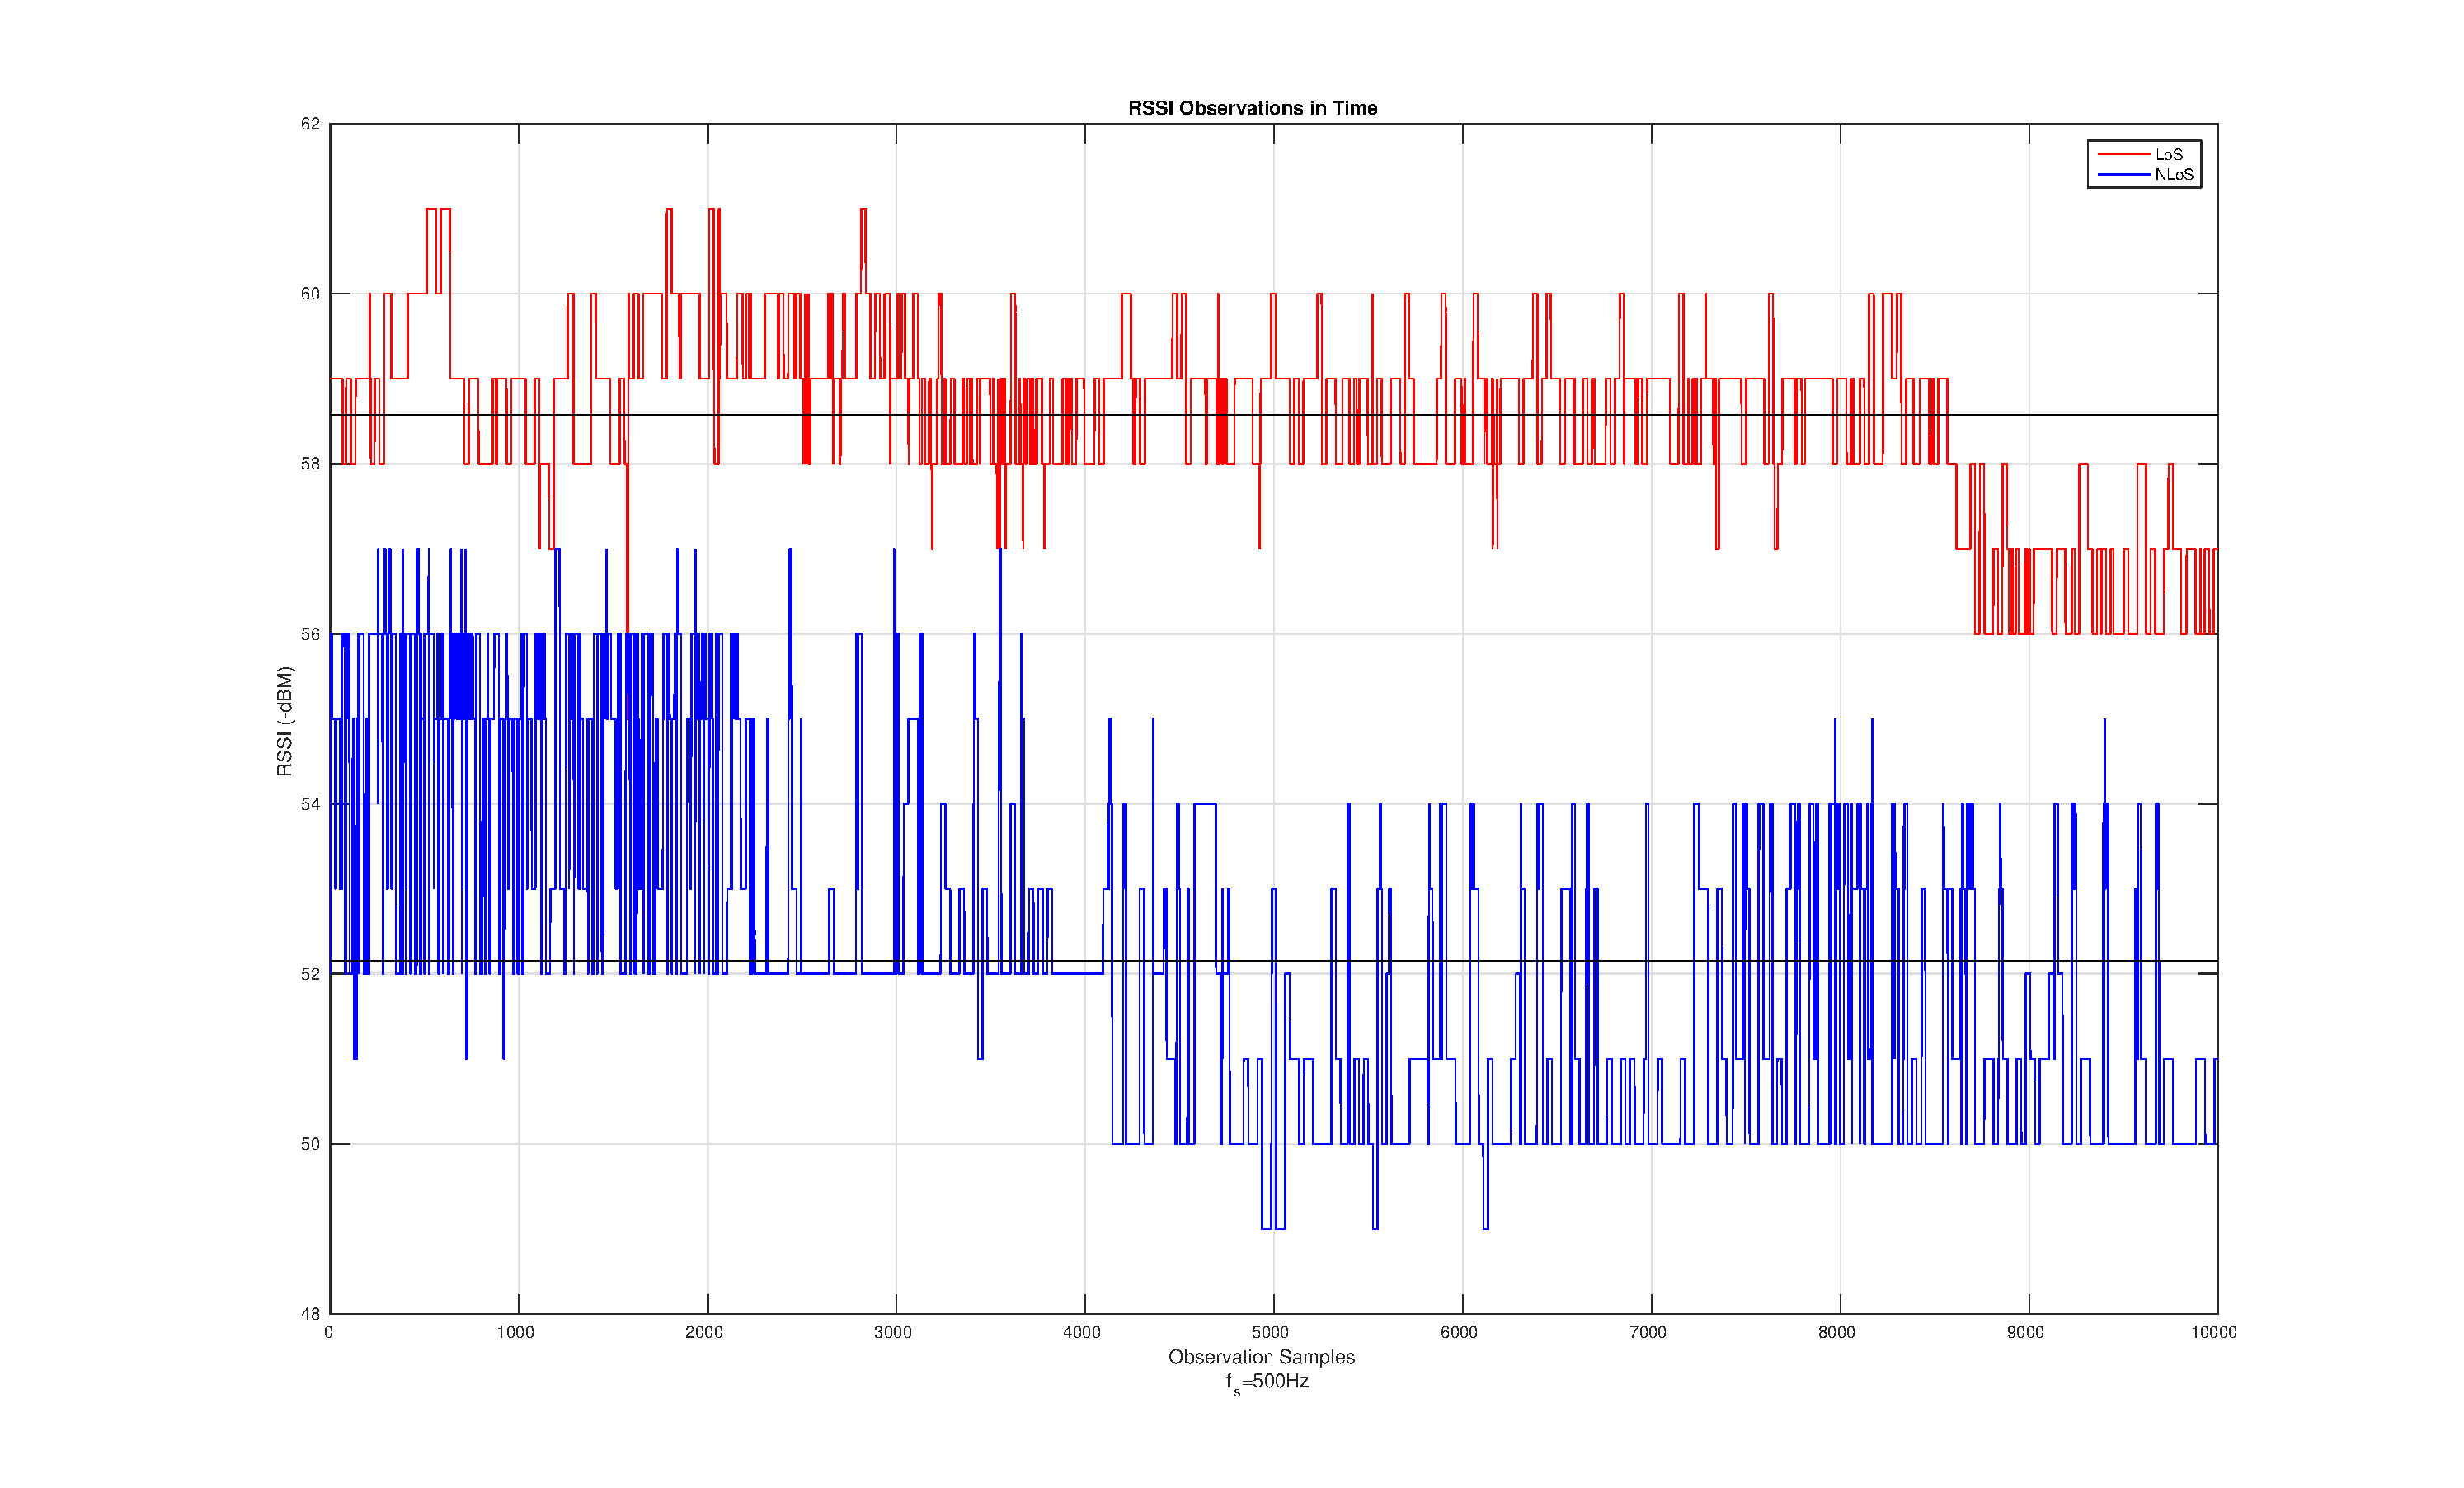
\includegraphics[scale=0.2]{figures/rssi_variance.eps}
         \caption{\label{fig-variance}RSSI readings of NLoS and LoS AP's acquired with a stationary agent}
      \end{figure}

  % \begin{itemize}
  %   \item CSI-related special \\
  %     hardware requirement
  %   \item Propagation-modelling \\
  %     multi-path effect difficult to model
  %   \item Fingerprinting \\
  %     An emerging area learning fingerprints is deep learning~\cite{gao2015channel}
  % \end{itemize}



  \section{\label{sec-PF}PROBLEM FORMULATION}

  \section{\label{sec-SD}SYSTEM DESCRIPTION}
    \subsection{Offline Stage}

      \subsubsection{Data Acquisition}

      \subsubsection{Training}

    \subsection{Online Stage}

      \subsubsection{Inference}

      \subsubsection{Information Fusion}


  \section{\label{sec-EX}EXPERIMENTATION}
    \subsection{Experimental Setup}
      \subsubsection{Hardware}
        Fetch~\cite{ackerman2015fetch}
      \subsubsection{Software}
        ROS~\cite{quigley2009ros}, Caffe~\cite{jia2014caffe}
    \subsection{Results}



  \section{\label{sec-CO}CONCLUSIONS}

  \section*{ACKNOWLEDGMENT}
  Turkish Government and stuff

  \bibliographystyle{IEEEtran}
  \bibliography{bibliography}


% An example of a floating figure using the graphicx package.
% Note that \label must occur AFTER (or within) \caption.
% For figures, \caption should occur after the \includegraphics.
% Note that IEEEtran v1.7 and later has special internal code that
% is designed to preserve the operation of \label within \caption
% even when the captionsoff option is in effect. However, because
% of issues like this, it may be the safest practice to put all your
% \label just after \caption rather than within \caption{}.
%
% Reminder: the "draftcls" or "draftclsnofoot", not "draft", class
% option should be used if it is desired that the figures are to be
% displayed while in draft mode.
%
%\begin{figure}[!t]
%\centering
%\includegraphics[width=2.5in]{myfigure}
% where an .eps filename suffix will be assumed under latex,
% and a .pdf suffix will be assumed for pdflatex; or what has been declared
% via \DeclareGraphicsExtensions.
%\caption{Simulation results for the network.}
%\label{fig_sim}
%\end{figure}

% Note that the IEEE typically puts floats only at the top, even when this
% results in a large percentage of a column being occupied by floats.


% An example of a double column floating figure using two subfigures.
% (The subfig.sty package must be loaded for this to work.)
% The subfigure \label commands are set within each subfloat command,
% and the \label for the overall figure must come after \caption.
% \hfil is used as a separator to get equal spacing.
% Watch out that the combined width of all the subfigures on a
% line do not exceed the text width or a line break will occur.
%
%\begin{figure*}[!t]
%\centering
%\subfloat[Case I]{\includegraphics[width=2.5in]{box}%
%\label{fig_first_case}}
%\hfil
%\subfloat[Case II]{\includegraphics[width=2.5in]{box}%
%\label{fig_second_case}}
%\caption{Simulation results for the network.}
%\label{fig_sim}
%\end{figure*}
%
% Note that often IEEE papers with subfigures do not employ subfigure
% captions (using the optional argument to \subfloat[]), but instead will
% reference/describe all of them (a), (b), etc., within the main caption.
% Be aware that for subfig.sty to generate the (a), (b), etc., subfigure
% labels, the optional argument to \subfloat must be present. If a
% subcaption is not desired, just leave its contents blank,
% e.g., \subfloat[].


% An example of a floating table. Note that, for IEEE style tables, the
% \caption command should come BEFORE the table and, given that table
% captions serve much like titles, are usually capitalized except for words
% such as a, an, and, as, at, but, by, for, in, nor, of, on, or, the, to
% and up, which are usually not capitalized unless they are the first or
% last word of the caption. Table text will default to \footnotesize as
% the IEEE normally uses this smaller font for tables.
% The \label must come after \caption as always.
%
%\begin{table}[!t]
%% increase table row spacing, adjust to taste
%\renewcommand{\arraystretch}{1.3}
% if using array.sty, it might be a good idea to tweak the value of
% \extrarowheight as needed to properly center the text within the cells
%\caption{An Example of a Table}
%\label{table_example}
%\centering
%% Some packages, such as MDW tools, offer better commands for making tables
%% than the plain LaTeX2e tabular which is used here.
%\begin{tabular}{|c||c|}
%\hline
%One & Two\\
%\hline
%Three & Four\\
%\hline
%\end{tabular}
%\end{table}


% Note that the IEEE does not put floats in the very first column
% - or typically anywhere on the first page for that matter. Also,
% in-text middle ("here") positioning is typically not used, but it
% is allowed and encouraged for Computer Society conferences (but
% not Computer Society journals). Most IEEE journals/conferences use
% top floats exclusively.
% Note that, LaTeX2e, unlike IEEE journals/conferences, places
% footnotes above bottom floats. This can be corrected via the
% \fnbelowfloat command of the stfloats package.
% trigger a \newpage just before the given reference
% number - used to balance the columns on the last page
% adjust value as needed - may need to be readjusted if
% the document is modified later
%\IEEEtriggeratref{8}
% The "triggered" command can be changed if desired:
%\IEEEtriggercmd{\enlargethispage{-5in}}

% references section

% can use a bibliography generated by BibTeX as a .bbl file
% BibTeX documentation can be easily obtained at:
% http://mirror.ctan.org/biblio/bibtex/contrib/doc/
% The IEEEtran BibTeX style support page is at:
% http://www.michaelshell.org/tex/ieeetran/bibtex/
%\bibliographystyle{IEEEtran}
% argument is your BibTeX string definitions and bibliography database(s)
%\bibliography{IEEEabrv,../bib/paper}
%
% <OR> manually copy in the resultant .bbl file
% set second argument of \begin to the number of references
% (used to reserve space for the reference number labels box)
% that's all folks
\end{document}
